\chapter{Introduction}

\section{Background}
As human spaceflight technology advances, we are entering a new era of exploration, moving from Earth into the cosmos. Ambitious initiatives such as NASA's Artemis program~\cite{NASA:2024acr} and SpaceX Mars colonization program~\cite{Musk:2017} signal a future where humanity may establish permanent bases on other celestial bodies and even achieve interplanetary colonization. However, realizing this grand vision hinges on the establishment of a stable and reliable interplanetary communication infrastructure.

The traditional Internet Protocol suite (TCP/IP), while exceptionally effective on Earth, is ill-suited for deep-space communication. Interplanetary networks face extreme challenges, including immense communication delays, extremely low bandwidth, and frequent link disruptions. These characteristics render the conventional end-to-end, real-time connection model virtually inoperable. To address these issues, academia and industry have proposed the concept of Delay-Tolerant Networking (DTN)~\cite{DTN}\cite{rfc4838}. The core principle of DTN is the "store-carry-forward" mechanism, which does not rely on persistent, real-time connections. Instead, it leverages the physical movement of network nodes—such as spacecraft, orbital satellites, or planetary bases—to buffer and transport data, thereby enabling reliable data transmission in extreme environments.

\section{Motivation}
Although DTN is widely recognized as the theoretical foundation for interplanetary communication, its practical application and deployment have lagged. The significant differences between the DTN protocol stack and existing internet infrastructure present a "reinventing the wheel" challenge for developers, requiring them to not only design the application layer but also to reconstruct the underlying network architecture. To overcome this barrier, researchers have made several key efforts:

\begin{itemize}
  \item Modular Protocol Design: The DTN stack, featuring the Bundle Protocol (BP) at its core, is designed with a modular architecture. This allows it to be flexibly integrated with various underlying transport protocols (e.g., TCP, UDP, or specific radio frequency protocols), thereby reducing development complexity. DTN architecture is given in Figure \ref{DTN_stack}.
  \begin{figure}[h]
      \centering
      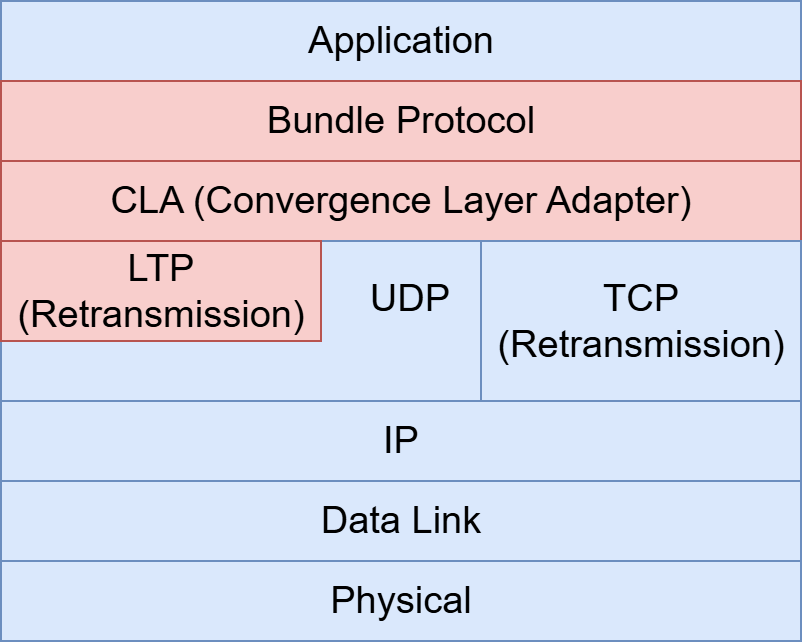
\includegraphics[width=0.6\linewidth]{introduction/DTN_stack.png}
      \caption{DTN stack}
      \label{DTN_stack}
  \end{figure}
  \item Integration with Existing Networks: Research efforts have focused on enabling the coexistence of DTN and traditional TCP/IP networks. For instance, DTN gateways can facilitate seamless data forwarding between the two network types, allowing DTN-enabled devices to access some existing network services and reducing the cost of rebuilding infrastructure.
\end{itemize}

Within the DTN application layer, email stands out as one of the most fundamental and critical communication tools. Its implementation in DTN environments has thus received considerable attention. Researchers have aimed to design a solution that leverages the advantages of DTN while maintaining compatibility with the existing email ecosystem. The IETF draft draft-johnson-dtn-interplanetary-smtp~\cite{draft-johnson-dtn-interplanetary-smtp} represents a significant attempt to create such a solution. This draft proposes a method for operating an SMTP service in a DTN environment, providing a valuable blueprint for translating theoretical concepts into practical, research-oriented applications.

\section{Research Question and Objectives}
This dissertation aims to conduct a systematic simulation and analysis of the Johnson Draft to answer the following core questions: Is the proposed scheme feasible in a simulated deep-space environment? What are its potential design limitations and shortcomings?

To achieve this goal, this dissertation will undertake the following specific objectives:

\begin{itemize}
  \item Construct a DTN Simulation Environment
  
  To build a software-based simulation platform capable of modeling the characteristics of deep-space communication, including high latency, low bandwidth, and intermittent link disruptions, thereby providing a foundation for subsequent experiments.

  \item Implement a DTN Email Service
  
  To develop a prototype of a delay-tolerant email service based on the Johnson Draft, enabling the functions of message sending, storage, forwarding, and reception within the simulation environment.

  \item Design and Execute a Validation Scenario
  
  To design a specific use case, such as an astronaut relocating from a Moon base to a Earth base and attempting to continue using the network for email communication. This scenario will be used to conduct a functional validation and performance assessment of the Johnson Draft.

  \item Analyze and Evaluate: To collect and analyze key performance metrics, such as average message delivery delay and success rate. Based on these results, this dissertation will conduct an in-depth analysis of the scheme's strengths and weaknesses concerning message ordering, data integrity, security, and resource management, identifying limitations that may arise in practical deployments.
\end{itemize}

Ultimately, this dissertation will not only validate the feasibility of the Johnson Draft but will also provide valuable insights for the design and optimization of future DTN applications, contributing to the effort of building a true interplanetary communication network.

\section{Dissertation Overview}
This dissertation is organized into six chapters. Chapter 1 provides an introduction to the research background, motivation, and objectives. Chapter 2 presents a literature review of related work in Delay-Tolerant Networking and its applications. Chapter 3 details the system design of the simulation platform. Chapter 4 describes the specific implementation and deployment of the system. Chapter 5 presents and discusses the experimental results. Finally, Chapter 6 concludes the dissertation and suggests directions for future work.